\documentclass[sigconf,nonacm]{acmart}
\settopmatter{printfolios=true}
\usepackage{booktabs,graphicx,listings,tikz}
\usetikzlibrary{positioning,arrows.meta}
\lstset{basicstyle=\ttfamily\scriptsize,breaklines=true,columns=fullflexible,showstringspaces=false,frame=single,aboveskip=4pt,belowskip=4pt}
\begin{document}
\title{ProduCast: From Relational Film Credits to a Semantic Knowledge Graph}
\titlenote{Repository: \url{https://github.com/karanbe17/film-talent-kg}}
\author{Karan Brahmbhatt}\affiliation{\institution{University of Victoria}\city{Victoria}\state{BC}\country{Canada}}\email{karanbrahmbhatt@uvic.ca}
\author{Moksh Patel}\affiliation{\institution{University of Victoria}\city{Victoria}\state{BC}\country{Canada}}\email{mokshpatel@uvic.ca}
\begin{abstract}
ProduCast represents film casting and production relationships as an RDF knowledge graph derived from a conceptual ER model and a revised relational catalogue. The ontology models overlapping talent professions, studios, award wins and performance roles. A curated sample replaces incomplete earlier film credits. A multi-page server-rendered interface accesses a Virtuoso SPARQL adapter with an embedded fallback. We provide a reproducible conversion, sample graph, ontology, query scripts and tests. Code: \url{https://github.com/karanbe17/film-talent-kg}.
\end{abstract}
\maketitle
\section{Conceptual and relational mapping}
The goal is to preserve the meaning of film credits while allowing linked data exploration. We follow the course progression from conceptual modeling to relational representation and then RDF/OWL~\cite{manual}. Figure~\ref{fig:er} retains the conceptual ERD without artificial surrogate ID attributes. The historical relational application is retained; the revised staging schema uses keys. Names and titles are useful labels, but do not globally identify individuals; the diagram's underlined labels reflect simplifying domain assumptions. We do not declare them as OWL keys.
\begin{figure}[h]
\centering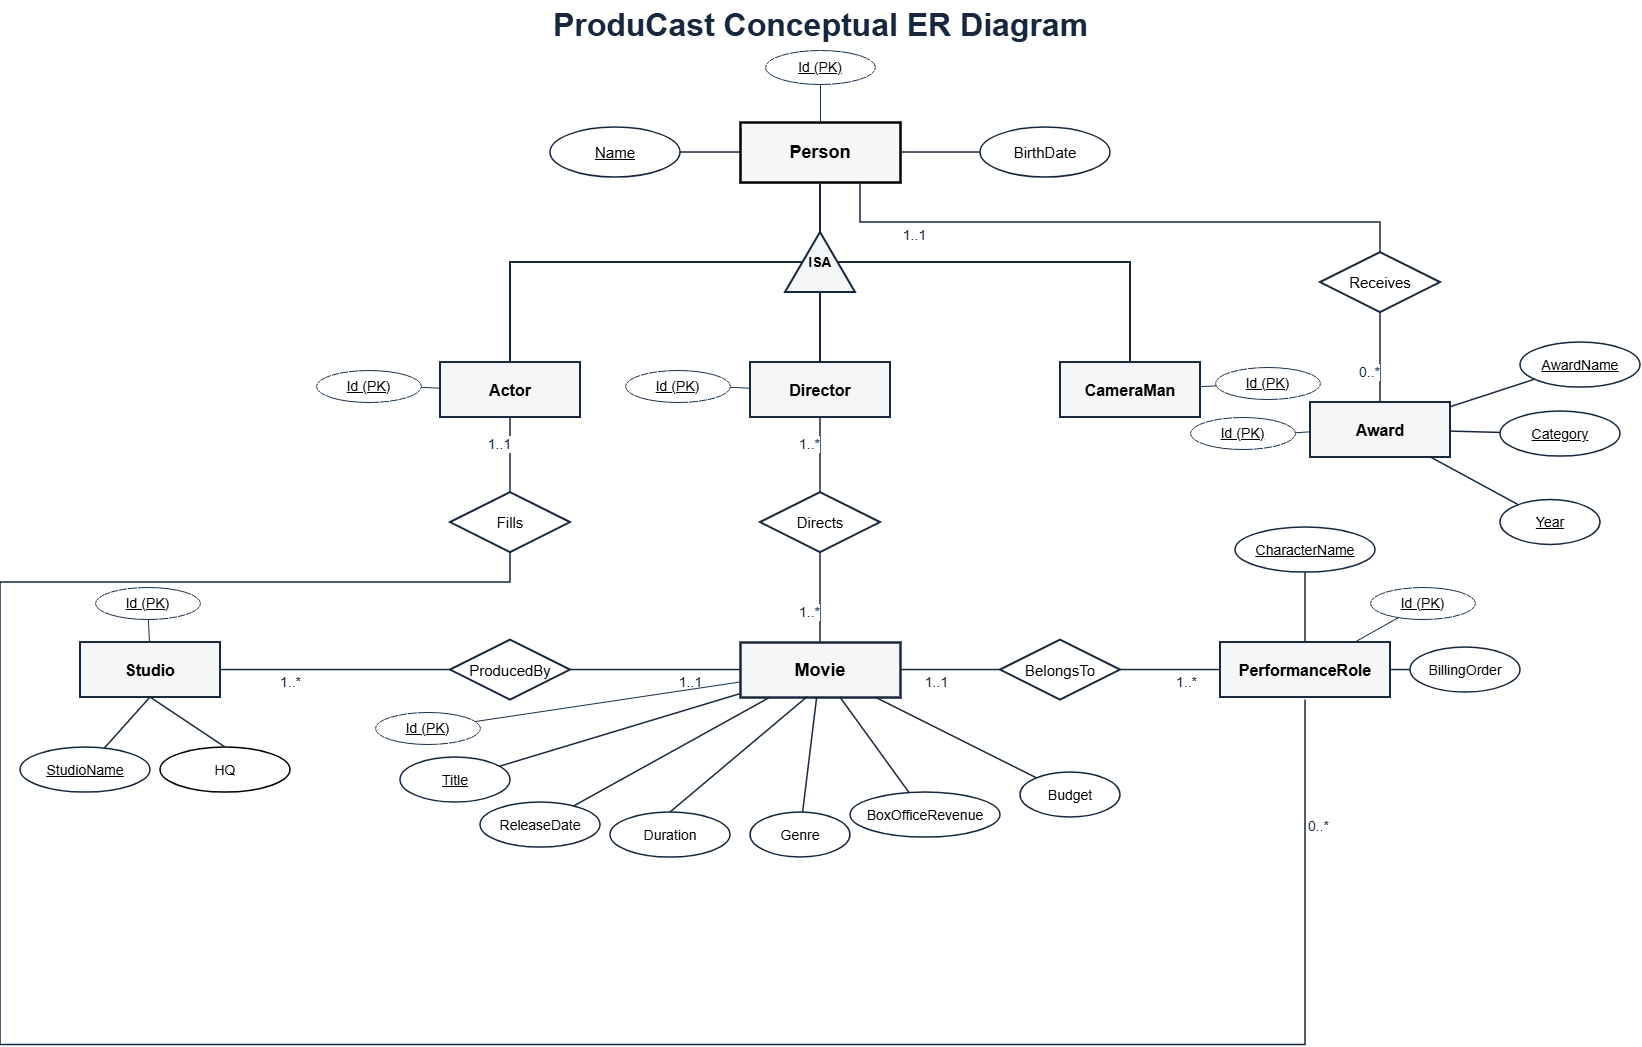
\includegraphics[width=\columnwidth]{er/ProduCast_ER_Diagram.png}
\Description{Chen ER diagram showing film entities and attributes without artificial identifiers.}\caption{Conceptual ER model (no surrogate IDs).}\label{fig:er}
\end{figure}
The converter builds a new normalized SQLite staging database from two curated text tables; the earlier database remains intact. The source tables contain films, people, professions, studios, credits and award occurrences. Stable staging keys become resource IRIs; overlapping professions share one individual. Director and cinematographer join tables map to object properties. PerformanceRole remains an association class because the character name belongs to a specific credit. The catalogue is a selected sample, not exhaustive filmographies.
\begin{table}[h]
\caption{Relational-to-RDF mapping.}\label{tab:map}
\small\begin{tabular}{@{}lp{1.85in}@{}}\toprule
Source & Semantic representation\\\midrule
Person & Person instance; name literal\\
Profession & Additional type on Person IRI\\
Movie & Movie instance; title and genre\\
Studio & Studio IRI; producedBy link\\
MovieDirector/Camera & directedBy / filmedBy\\
PerformanceRole & Role instance; filledBy, belongsTo, characterName\\
Award & receivedBy, awardedFor, category, year\\\bottomrule\end{tabular}
\end{table}
\section{Ontology design}
RDF~\cite{rdf} expresses facts as subject--predicate--object triples. RDFS and OWL~\cite{owl} describe vocabulary and semantics (TBox), while instance triples form the ABox. Eight classes represent the ER entity sets: Person, Actor, Director, CameraMan, Movie, Studio, Award and PerformanceRole. Actor, Director and CameraMan are subclasses of Person and may overlap. Datatype properties cover names, dates, film duration, financial attributes, year, role and billing order. Object properties connect films to studios/directors and roles to films/actors; awards link to a recipient and the winning film. Inverse properties express the converse relationships. We add \texttt{filmedBy} and \texttt{awardedFor} as explicit extensions of the conceptual baseline. Release year is recorded when exact dates are unknown. Table~\ref{tab:rules} summarizes the restrictions.
\begin{table}[h]
\caption{Selected OWL restrictions and types.}\label{tab:rules}
\small\begin{tabular}{@{}lp{1.66in}@{}}\toprule
Property & Constraint / range\\\midrule
producedBy & Movie: exactly 1 Studio\\
directedBy & Movie: at least 1 Director\\
belongsTo, filledBy & Role: exactly 1 Movie and Actor\\
receivedBy & Award: exactly 1 Person\\
hasRole & Movie: at least 1 role\\
roleType & Lead, Supporting or Cameo\\
birthDate, releaseDate & xsd:date\\
duration, billingOrder & xsd:positiveInteger\\\bottomrule\end{tabular}
\end{table}
\clearpage
\section{Knowledge graph and implementation}
The revised sample contains 35 films, 43 actors, 31 directors, 31 cinematographers (104 distinct people), 29 selected production companies, 59 performance roles and 82 award wins. The seed has 1,771 explicit instance triples and 193 ontology triples. Each film has cast, director, studio and camera links; every actor has a role. The Academy and Golden Globes archives provide award review references~\cite{oscars,globes}; film credit review links and scope are documented in the repository. Not every fact has been independently verified. Unknown dates, budgets and classifications are omitted. The ontology is generated programmatically and its RDF/XML syntax and structure were validated.
\begin{figure}[h]
\centering
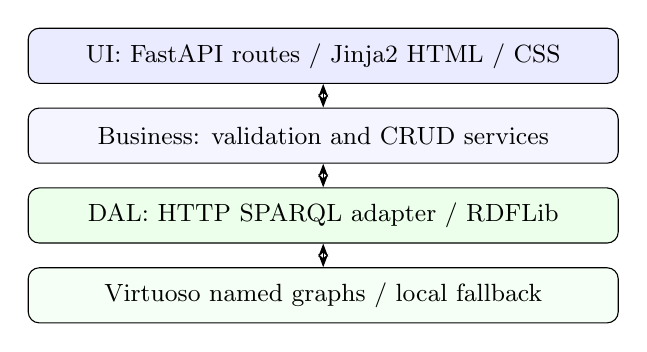
\begin{tikzpicture}[node distance=3mm,>=Stealth, every node/.style={font=\small},layer/.style={draw,rounded corners,align=center,minimum width=2.95in,minimum height=7mm}]
\node[layer,fill=blue!8] (ui) {UI: FastAPI routes / Jinja2 HTML / CSS};
\node[layer,fill=blue!4,below=of ui] (biz) {Business: validation and CRUD services};
\node[layer,fill=green!8,below=of biz] (dal) {DAL: HTTP SPARQL adapter / RDFLib};
\node[layer,fill=green!4,below=of dal] (rdf) {Virtuoso named graphs / local fallback};
\draw[<->] (ui)--(biz);\draw[<->] (biz)--(dal);\draw[<->] (dal)--(rdf);
\end{tikzpicture}
\Description{Four layers: browser-facing UI, business services, data access layer and persistent RDF graph.}\caption{Semantic application layers. SQLite is read during seed conversion only.}\label{fig:arch}
\end{figure}
The Virtuoso adapter sends SELECT and scoped SPARQL updates to the authenticated server endpoint. RDFLib~\cite{rdflib} converts the revised SQLite staging database and stages input validation; the server persists separate schema and data graphs. An embedded RDF/XML fallback is retained. The original Flask/SQLite app is unchanged; the semantic application uses FastAPI, Jinja2 and local CSS. Figure~\ref{fig:arch} shows the architecture. The adapter is designed for a single writer and a small demonstration dataset. A Docker Compose configuration, RDF/XML and standalone SPARQL files support reproducible setup. Live verification on the merged repository successfully loaded both named graphs and executed SELECT, INSERT, UPDATE and DELETE.
\subsection{From schema to instance triples}
The ontology states that CameraMan is a subclass of Person. Instance types are explicit, since no reasoner runs at query time. The abridged Turtle example illustrates a film and cinematographer; illustrative resource names stand for the generated IRIs.
\begin{lstlisting}
pc:CameraMan rdfs:subClassOf pc:Person .
pc:cameraExample a pc:CameraMan, pc:Person ;
 pc:name "Hoyte van Hoytema" .
pc:movieExample a pc:Movie ;
 pc:title "Oppenheimer" ;
 pc:filmedBy pc:cameraExample .
\end{lstlisting}
The converter uses the same resource identifier whenever a person appears in multiple credits. This makes cross-film traversal possible without relying on textual name joins. The generated RDF/XML files can be loaded independently of the web application, enabling inspection and reuse by other semantic tools. The schema and instance graphs can also be queried separately, so the application does not confuse class declarations with catalogue records.
\newpage
\section{SPARQL data manipulation}
SPARQL~\cite{sparql,update} matches graph patterns rather than tables. A movie--actor query traverses the association resource, preserving the character name. For brevity the examples use the namespace prefix defined below.
\begin{lstlisting}
PREFIX pc: <https://github.com/karanbe17/film-talent-kg/ontology#>
\end{lstlisting}
\begin{lstlisting}
SELECT ?movie ?actor ?character WHERE {
 ?r pc:belongsTo/pc:title ?movie;
    pc:filledBy/pc:name ?actor;
    pc:characterName ?character .
}
ORDER BY ?movie ?actor
\end{lstlisting}
The result includes 59 role credits, e.g., Rocky / Sylvester Stallone / Rocky Balboa and Inception / Leonardo DiCaprio / Dom Cobb. Collaboration counts group by resource IRIs to avoid merging people with matching labels. Studio aggregation, awards, cinematography and overlapping professions provide complementary queries.
\begin{lstlisting}
SELECT ?person (COUNT(DISTINCT ?role)
 AS ?professions) WHERE {
 ?p a pc:Person; pc:name ?person; a ?role .
 VALUES ?role {pc:Actor pc:Director pc:CameraMan}
} GROUP BY ?p ?person
HAVING(COUNT(DISTINCT ?role)>1)
\end{lstlisting}
The current graph returns Denzel Washington with two professions. The DML demonstration uses an isolated scratch graph to insert, rename and delete a temporary individual; it asserts that the expected name is returned before and after the update, and no row remains after deletion.
\begin{lstlisting}
INSERT DATA { pc:temporary-demo a pc:Person;
 pc:name "Temporary Demo" . }
DELETE { pc:temporary-demo pc:name ?old }
INSERT { pc:temporary-demo pc:name "Updated Demo" }
WHERE  { pc:temporary-demo pc:name ?old }
DELETE WHERE { pc:temporary-demo ?p ?o }
\end{lstlisting}
\begin{table}[h]
\caption{Executed SELECT results on the seed graph.}\label{tab:results}
\small\begin{tabular}{@{}lr@{}}\toprule
Query & Rows\\\midrule
Cast by film & 59\\
Actor--director collaborations & 58\\
Studio film counts & 29\\
Award recipients & 82\\
Camera credits & 35\\
Overlapping professions & 1\\\bottomrule\end{tabular}
\end{table}
\subsection{Live database verification}
The verification script loads the ontology and instance graph into disposable named graphs and compares their sizes with the RDF/XML source files. It executes the prepared queries, then checks insertion, modification and deletion of a temporary resource. The live run returned 29 studio rows, 82 award rows, 35 camera-credit rows and one overlapping-profession row. All graph-loading and DML assertions passed. The separate local DML demonstration also confirmed that the original data remained unchanged. These checks establish operational reproducibility for the supplied sample rather than completeness of the real-world catalogue.
\clearpage
\section{User interface and evaluation}
ProduCast offers separate Overview, Movies, Talent, Studios, Awards, Casting and Collaborations pages. Talent has actor/director/cinematographer filters, portfolios with characters, awards and shared films. Technical queries are available under Research tools. Users search and use validated forms rather than entering SPARQL. The UI supports creation, modification and deletion for all five record categories. Talent profession selection supports multiple roles. A new casting record requires a valid movie and actor. Invalid role types and invalid referenced individuals are rejected. Deleting a movie removes dependent role and award individuals; deleting a person also removes their role and award records and incoming credits. An in-use studio cannot be deleted. These are application-level choices rather than OWL entailments.
\begin{figure}[h]
\centering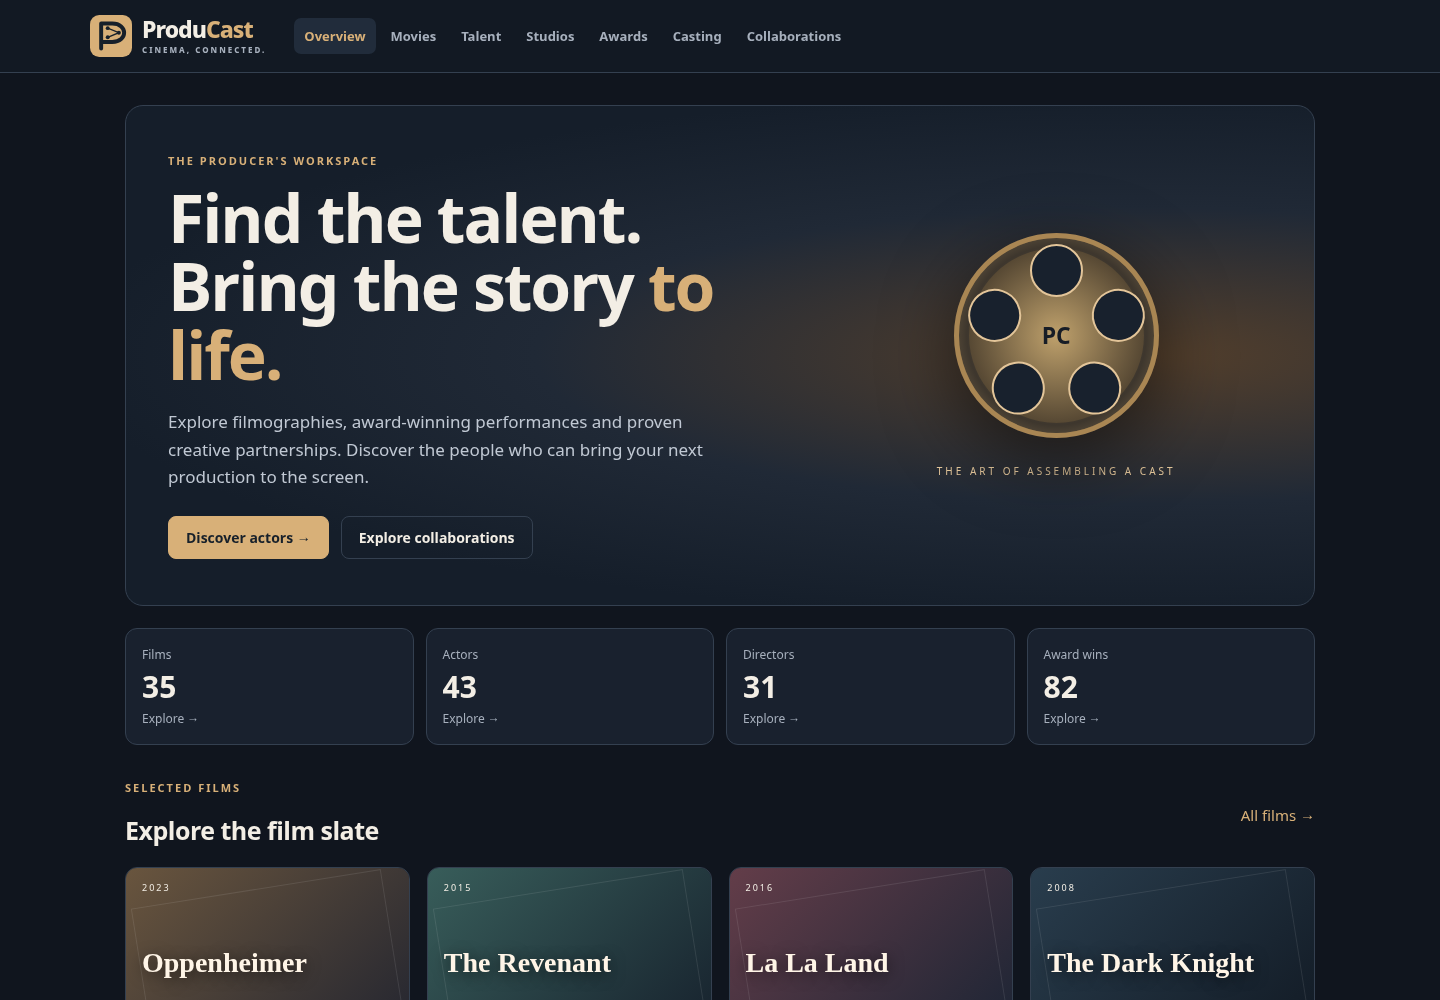
\includegraphics[width=\columnwidth]{semantic_screenshots/overview.png}
\Description{Dark cinema-themed producer workspace with film cards and catalogue statistics.}\caption{Overview rendered from the implemented application.}\label{fig:ui}
\end{figure}
\begin{figure}[h]
\centering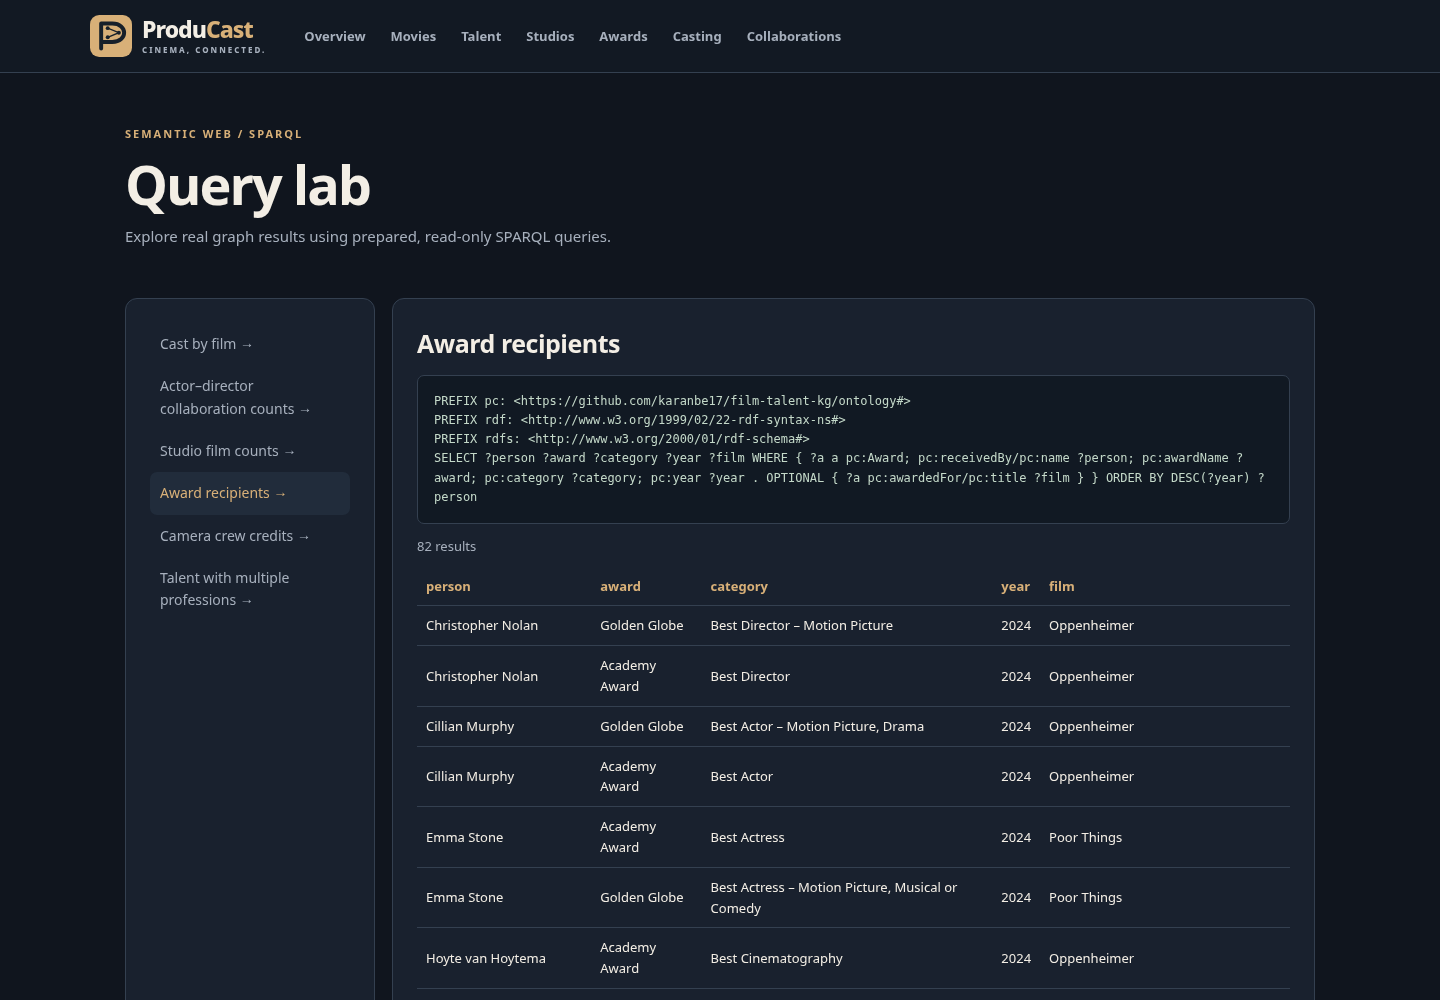
\includegraphics[width=\columnwidth]{semantic_screenshots/query.png}
\Description{Query lab showing a SPARQL statement and award query results.}\caption{Prepared SPARQL query and results (application render).}\label{fig:query}
\end{figure}
OWL adopts the open-world assumption: an absent statement is not necessarily false. We distinguish logical restrictions from validation. The seed passes movie-link coverage checks; missing wins are not evidence that a person has never won an award. Minimum participation is not fully enforced during incremental entry. No automatic OWL reasoner or formal closed-world validation engine is enabled. One selected production company per film is recorded, not all producers. The curated catalogue is not a verified comprehensive industry dataset.
\section{Reproducibility and limitations}
The repository includes pinned Python dependencies, Docker Compose, RDF/XML, SPARQL scripts and quickstart documentation. After starting Virtuoso and setting the local password, run \texttt{python verify\_virtuoso.py} and start the app with the \texttt{-{}-virtuoso} flag. The verification script uses disposable named graphs. Omitting the flag selects the embedded fallback. Five automated cases passed, including a simulated server protocol. Live Virtuoso graph loading and all four SPARQL operations passed; the standalone DML demonstration preserved the original data. The website and quickstart were successfully executed on the merged repository by Karan. The application supports search, linked portfolios, a Collaborations view, CRUD and export. Screenshots show the embedded test rendering, not a live Virtuoso session. The application is local and unauthenticated, not a production service. Findability is supported by the repository and stable IRIs; accessibility by documented setup; interoperability by RDF/XML, OWL and SPARQL; and reuse by source data, conversion scripts and tests~\cite{fair}.
\section{AI disclosure}
ChatGPT~\cite{ai} assisted in generating the implementation, ontology, tests, interface, and draft report. The repository documents AI task completion (level D). Karan reproduced the backend tests, live Virtuoso operations and quickstart, checked the website and integrated the backend changes. Moksh integrated the frontend changes on his own branch. These activities are distinct from AI generation; no full OWL reasoner or independent verification of every credit is claimed.
\begin{thebibliography}{9}
\bibitem{manual} University of Victoria. 2026. CSC501 Project Manual, Milestone 5: Semantic Web.
\bibitem{rdf} W3C. 2014. RDF 1.1 Concepts and Abstract Syntax. \url{https://www.w3.org/TR/rdf11-concepts/}.
\bibitem{owl} W3C. 2012. OWL 2 Web Ontology Language Primer. \url{https://www.w3.org/TR/owl2-primer/}.
\bibitem{rdflib} RDFLib developers. RDFLib documentation. \url{https://rdflib.readthedocs.io/}.
\bibitem{sparql} W3C. 2013. SPARQL 1.1 Query Language. \url{https://www.w3.org/TR/sparql11-query/}.
\bibitem{update} W3C. 2013. SPARQL 1.1 Update. \url{https://www.w3.org/TR/sparql11-update/}.
\bibitem{fair} M. D. Wilkinson et al. 2016. The FAIR Guiding Principles for scientific data management and stewardship. \textit{Scientific Data} 3, 160018.
\bibitem{oscars} Academy of Motion Picture Arts and Sciences. Ceremony archive. \url{https://www.oscars.org/oscars/ceremonies}.
\bibitem{globes} Golden Globes. Winners and nominees. \url{https://goldenglobes.com/winners-nominees/}.
\bibitem{ai} OpenAI. 2026. ChatGPT (GPT-6.2), project assistance, 24 November 2026.
\end{thebibliography}
\end{document}
